
Software Defined Networks (SDN) change the traditional model of network
architecture and design. Traditionally,  networking  relied and evolved over a non-transparent distributed model for
the deployment  of  protocols and configuration of devices. This model
lead to complex protocols and management functions. SDN presents a new way of thinking in networking,
shifting the complexity of protocols and management functions from  the  networks
devices to a general purpose logically centralized service. 

Historically  the network academic environment has followed an 
ad-hoc approach to networking where protocols are introduced as a
response to specific problems. Scoot
Shenker, a networking researcher from Berkley\footnote{Scoot Shenker has played a fundamental role in SDN development, collaborating in many papers. He is also co-founder of both ONF \cite{onf} and Nicira Networks - both very important to SDN.}, ironically sums up  this contribution to networking as a ``big bag of
protocols'' \cite{Shenker:2011ys}. In his opinion there is a lack of
\emph{control abstractions} in current network architectures that, allied  with  their  distributed nature,
lead to the  complex infrastructure available today. Additionally the
network field has failed to developed the appropriate tools for
managing such complexity. 

SDN breaks this complex model through the
physical detachment of the control and data planes.  The motivation behind this
decoupling is the following: if the distributed network state can be collected
and presented to a logically centralized service then it is simpler to both to
specify network level objectives as well as to translate these
objectives into the appropriate configuration of network devices. These
planes, when loosely coupled, can simplify the development of protocols
and the management of network infrastructures. 

In this section we present a historical perspective
of contributions leading to the standardization process of SDN and a
terminology/concept section necessary for
proper understanding of the remaining discussion in this document.  


\section{Software Defined Networks}
\glsresetall
\label{sec:background:sdn}
Software Defined Networking is a networking research field born from a  distributed
collaborative effort. In this section we
outline some of the major contributions that have
led to its current state. 

\subsection{Fundamentals} 
\subsubsection{4D.} The origins of SDN can be traced back to the 4D architecture published in  2005 that ``generated both broad consensus and wide disagreements from
the reviewers''  \cite{Greenberg:2005boa}. In this seminal work the authors identify essential
problems governing  the traditional network architecture and  present an
explanation of the design process behind a clean-slate architectural
pattern for  the development of new networks. 

The authors identify  the root cause of the complexity inherent to the
classic Internet design as the  entanglement  of control and
forwarding functions in the network devices. They advocate that this complexity is tied to the lack of accessible control abstractions in the network devices. 

 With this in mind they present the  4D architecture. Their  design is led by the
decoupling of the control plane from the data plane. Additionally, they
identify three key requirements for the 4D architecture: specification of  network level goals (e.g., routing,
security policy);  centralization of the network state (e.g.,
topology) and finally; direct control of the underlying network
devices.

The 4D architecture can be seen
in Figure \ref{fig:4d}. A description of the four layers
follows: 

\begin{figure}
  \centering 
  \footnotesize
  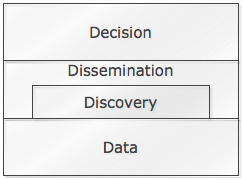
\includegraphics[scale=0.5]{pic/4d.png}
  \caption[The 4D architecture]{\textbf{The 4D architecture}: is
    composed by 4 planes. Notice that Discovery operates
  in the Dissemination plane.}
  \label{fig:4d}
\end{figure}

\begin{itemize}
\item[] \textbf{Decision:}  defines network-level goals and 
  translates them to configuration primitives of the network
  equipment. This plane maintains a representation of the current state of the network (i.e., the network view); 
\item[] \textbf{Dissemination:}  connects the Decision and Data plane. Must be
  done with robustness guarantees; 
\item[] \textbf{Discovery:} provides discovery information (e.g., network
  equipment, interfaces, etc.) from the Data plane to the Decision plane; 
\item[] \textbf{Data:}  is governed by the network equipment
  infrastructure. Provides packet forwarding functions and implements
  an interface to the Decision plane;  
\end{itemize}

4D effectively removes network logic  from the Data plane
responsibilities. It advocates that what was previously done through complex
routing protocols and per-box configurations (e.g., security policy
definitions)  can be specified in the Decision plane. 

The 4D architecture, even without a concrete implementation, 
presented a significant mark in the history of SDN by setting the
ground for discussion and evolution focused on this essential
decoupling of control and data planes.  

\subsubsection{Ethane.}Ethane \cite{Casado:2007kb} was published in 2007 and presents a
network architecture for the enterprise with emphasis in
security. This work adapts the 4D design to implement a centralized
high-level security policy manager in the controller allied with a namespace  for users and nodes
available in the Network Information base (NIB). The Decision plane is also responsible for
authentication of both users and nodes. 

In Ethane the 4D Decision plane  is instantiated in a complex software
running in a server named \emph{controller}. The controller guarantees
that the security policy is respected. To do so, it can manipulate the network
devices available in the network. The devices perform  flow-based
forwarding  with the help of a local  flow table that is maintained by the
controller. Every flow that fails to match with any of the rules
available in the flow table  is redirected to the controller. After the
control logic is applied the controller may perform several actions
including: forwarding/flooding the packet;  installing flows in the
switch;  drop the packet; etc., The controller plays the interposition role
between any two pair of hosts. The security policy is defined over
high-level names. As
authentication is performed in the controller it is easy to maintain
bindings between these names and dynamic addresses. 

In the paper several replication techniques are presented 
as possibilities for ensuring fault tolerance of the Ethane controller. These are the following: 

\begin{itemize}
\item[] \textbf{Cold standby:}  In this mode backup controllers are passive entities
  waiting to take over if  the active controller fails. Backup
  controllers participate in the
  Minimum Spanning Tree (MST) protocol where the active controller  is
  defined as the root of the tree. Upon failure of the active
  controller the tree converges to a new root (i.e., a new
  controller). Replication only covers authentication and
  network security policy state with simple (unspecified) consistency
  properties that are not strong enough to avoid requiring 
  re-authentication of a subset of  the users when the active
  controller fails. 
\item[] \textbf{Warm-Standby:} In this case  passive controllers recovery
  faster as separate  MST's are maintained for every controller. In this replication
  method the authors also replicate bindings across
  Controllers. However, 
  these are replicated with weak consistency and as so, may require
  re-authentication from users or nodes upon failure of the active controller.

\item[] \textbf{Fully-Replicated}: In this approach two or more active
  controllers are fully replicated. The authors advocate the use 
  of weak-consistent methods based on gossiping but also leave 
  the study open for the use of a fully replicated state machine.
\end{itemize}

Ethane major contribution comes from the practical  experience with
the deployment in the Stanford
University  campus network. The  analysis performed suggests that a single
desktop computer alone could handle a network with over 20K hosts. 

\subsubsection{OpenFlow.} Both Ethane \cite{Casado:2007kb} and 4D \cite{Greenberg:2005boa}
focused in the decoupling of the control plane from the data plane, however there is also required that the control plane can programatically define the data plane configuration. In Ethane this
feature was presented in a monolithic  implementation of the controller.
For general development of SDN  it is  necessary that a
standard interface is available. OpenFlow \cite{openflow}, published
in 2008,  was the first protocol enabling this interface by allowing
the remote manipulation of flow based forwarding network devices. 

OpenFlow (OF) is introduced in the context of an architecture similar to
Ethane \cite{Casado:2007kb}, in which network devices 
are also simple flow-based forwarding equipments. A flow
table resides in the network device and is composed of tuples
$\langle match,action \rangle$. The $match$ entry allows the device to match
arriving packets, while  $action$
specifies the forwarding behavior. Matches can be performed against
standard fields in Ethernet, IP and transport headers while actions can
range from dropping packets; forwarding to single port(s); and/or forwarding to controller. As in Ethane, a non-matching flow is forwarded to the controller who in
turn should instruct  the network device on future behavior through
the modification of the device flow table. Once the table is instructed, 
subsequent packet with matching headers can be forwarded without
the controller interaction. 

Currently the OpenFlow specification is maintained by the Open Network
Foundation (ONF). At the time of writing, the version 1.3 \cite{of13} is available with
several improvements over the original paper \cite{openflow}. 

\subsubsection{Network Operating System.} The Network Operating System (NOS) terminology  was initially used in the
context of Operating Systems (OS's) to name OS's with network services available. In the
context of SDN it was, to our knowledge,
introduced by Gude et al. \cite{Gude:2008jd} and
Cai et al. \cite{Z.-Cai:2008fk}. 

The role
of the Network Operating System is to provide
applications residing above it the ability to effectively control and
observe the state of the network. This ability is provided through a
programmatic interface defined in the Network Operating System itself and should be general
enough to support a broad spectrum of  network management
applications. With the help of this interface it is easier to define
and deploy network control applications such as firewalls and load
balancers. 

This functionality of a NOS is similar to conventional  Operating
Systems (OS's) with the fundamental difference of the managed resources. A
regular OS manages hardware devices from a computer 
and  a NOS manages a network.
The latter environment is harder to manage than the former. 
Aside this difference, the role of the NOS is to implement the
device drivers to communicate with the
network devices and also provide a platform for deployment of network
control applications with integration, communication and
isolation features (as a regular OS does for computational systems). 

In essence, this concept set a clear line in the separation of network applications
from configuration of network devices. The NOS abstraction brings different attributes to the development process of
network control functionality that, until now, was bound by the hardware and respective
software development cycle. Development is still bounded due to the
capabilities of the devices under management of the NOS but at least
the NOS itself and the applications can follow a software-only
development cycle. Additionally one can expect most of SDN functionality to be
heavily dependent   on the applications build on top of NOS much like
current  OS user level functionality is offered by applications
running outside the kernel.

%TODO - they can be a challenge to distributed controllers. 

\subsection{General Architecture}
In March 2011 the Open Network Foundation was created with the
participation and support from several industry partners \cite{onf}. ONF  is a ``non-profit consortium
dedicated to the transformation of networking through the development
and standardization of a unique architecture called Software-Defined
Networking (SDN)''. They have done so, by releasing a white-paper
defining the design principles for a SDN architecture and the
advantages of it \cite{ONF:2012ui}. They are also responsible for the standardization
process of the OpenFlow protocol.

It is important to emphasize that Software Defined Networks is not a
standard. It should be
clear, by now, that SDN's are an architectural pattern with two
essential properties:

\begin{itemize*}
\item Decoupling of the control plane from the data plane;
\item The network control must be driven by software.
\end{itemize*}

In this section we present the SDN architecture used as reference throughout this document.  

\subsubsection{General architecture.} The architecture of Software Defined Network is presented in Figure
\ref{fig:sdn-stack}. A bottom up explanation of the responsibilities of
each layer follows:

\begin{figure}
  \centering 
  \footnotesize
  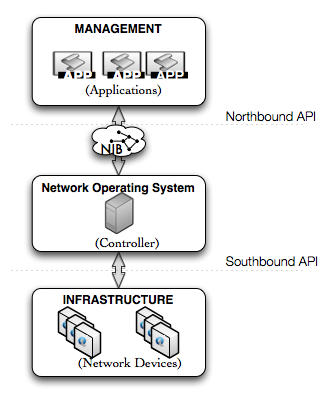
\includegraphics[scale=0.5]{pic/sdn-stack.png}
  \caption[SDN Architecture]{\textbf{SDN Architecture}: is composed by three
    layers: in \textbf{Management} resides the application
    logic that governs the overall network behavior; The
    \textbf{Network Operating System} (NOS)  allows the integration
    of  Management applications and exposes an interface for the
    manipulation of the network (northbound API). It also exposes the Network
    Information Based (NIB); Finally the network is
    represented in the \textbf{Infrastructure} layer. The devices must
  implement an interface allowing configuration (southbound API)}
  \label{fig:sdn-stack}
\end{figure}

\begin{itemize}
\item[] \textbf{Infrastructure Layer:} In this layer are the network
  devices responsible for packet forwarding. Any device 
  can be used (wireless access point, Ethernet switch, router) as long as it implements 
  a standard configuration interface (e.g., OpenFlow). Throughout the text we refer to all these devices as switches;
\item[] \textbf{Network Operating System (NOS):} Provides a standard
  interface to the upper layer (i.e., the northbound interface) allowing the manipulation of the network
  state such as forwarding tables in the managed devices. The
  configuration of devices is actually done by the NOS by interaction
  with the Infrastructure interface for configuration (i.e., the southbound interface). Additionally, it should provide features
  for the integration of Management layer applications.  Throughout
  the text we use NOS, controller or control plane to refer to this
  layer;
\item[] \textbf{Management:} This is where the network logic operates. In this layer
  resides the definition of network level objectives in the form of
  one or more applications. These applications interact with the NIB
  to consult and modify the network state. 
\end{itemize}

The NOS layer provides the northbound API to the upper layers. Network
applications run in the Management layer and can interact with the
network through this API. The NOS layer is also responsible for
communicating with the network devices through the southbound API. The
usual implementation of this API is the OpenFlow protocol.

Notice that the Network Operating System layer plays the intermediary
role in the stack. This implies that not only it allows that
Management applications alter the network state but  also has to
communicate to the Management layer the events that occur at the
Infrastructure level. Complex controllers such as Onix
\cite{Koponen:2010th} use the NIB as the intermediary in this duplex
communication while  the vast majority of controllers only use the NIB as a
simple datastore. 

There must be reliable connectivity between the Network Operating
System and the Infrastructure. The connectivity may be 
\textbf{in-bound} or \textbf{out-bound}
. In the in-bound case the connectivity takes place over the
network used for data forwarding while in the out-bound case a
different and isolated network is used. Connectivity
between these two layers require manual configuration of the
Infrastructure components. 

\subsubsection{Types of Controllers.} The controller is often
categorized in the literature
``logically centralized'' \cite{Gude:2008jd,Greenberg:2005boa}. This concept is used in distributed systems literature
to refer to a physically distributed system that appears, to
its users,  as a
coherent and  transparently distributed service (i.e., it does not
appears to be distributed). The term is perhaps
not well employed in SDN literature as pointed out in
a blog post, by Martin Casado, a Stanford researcher and Nicira
co-founder \cite{:zr}. We will not maintain
this terminology either. Instead, we define that the control platform is 
either  \textbf{distributed} or 
\textbf{centralized} for the remaining discussion. In the centralized
case a single controller is responsible for all the network
Infrastructure as opposed to the distributed case where several
controllers are used.

Another category  distinction in controller software is based on another text
from Casado and Koponen \cite{Martin-Casado:2011ly}, where
three categories of controllers are discussed: 

\begin{itemize}
\item[] \textbf{Single Purpose Controller:} lack support for general management
  applications. Ethane is an example of this type of controllers; 
\item[] \textbf{Thin Controller:} present a northbound interface that is
  strongly-coupled to the southbound interface. Most controllers fall
  under this category. Usually these controllers are known as OpenFlow controllers given the use of OpenFlow in the southbound interface.  
\item[] \textbf{General Controllers:} offer a general purpose service with loosely
  coupled south and northbound interfaces. Transition from the OpenFlow protocol for
  other protocol may  be completely transparent to the Management layer.
\end{itemize}



\section{Physically Centralized  Controllers}
\glsresetall
\label{sec:background:centralized}


In this section we present an overview of relevant centralized
controllers. Centralized controllers are, by our definition, control
planes that do not show any explicit support in the deployment of a
different controllers processes over onde or more servers. 
\subsection{Existent Controllers}
%TODO - what defines a centralized controller. 
%TODO - pipeline as a common model
%TODO - event based
%TODO - thin. 
\subsubsection{NOX}
\label{sec:nox}
NOX \cite{Gude:2008jd}  was published and publicly released under
GPL in 2008. It was both developed in C++ and Python. NOX enables a standard interface for the integration of  Management applications 
in the controller. These applications control
network objectives and also cooperate to define the current
network view (i.e., the NIB). The view is shared between applications. One of the
contributions of the article was the definition of the Network
Operating System abstraction for the controller service. However, NOX
is a Thin Controller. 

\begin{figure}
  \centering 
  \footnotesize
  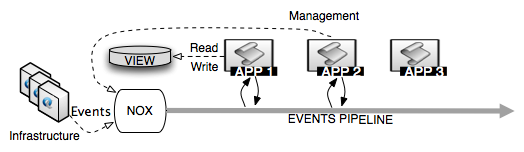
\includegraphics[scale=0.5]{pic/nox-pipeline}
  \caption[NOX pipeline] {\textbf{NOX pipeline} An overview of the NOX
    pipeline used for event processing by the Management applications. NOX
  receives events that have originated either in the Infrastructure of
the Management layer and dispatches them through a pipeline of
applications who have registered for processing these events. 
 As an example: \emph{PACKET\_IN} is a network event while
\emph{USER\_AUTHENTICATED} could be an application event.}
  \label{fig:nox-pipeline}
\end{figure}

NOX is a component framework with primitives for
construction and deconstruction of OpenFlow
based messages. The programming model is event-based. Applications (the components) are registered in a
priority based pipeline with event handlers associated to either
OpenFlow or applications events. This process can be seen in Figure
\ref{fig:nox-pipeline}, which describes the NOX dispatching behavior. Notice
that applications decide if the event should continue to be processed
by the pipeline. NOX  currently ships
with several applications (e.g., forwarding, topology discovery, host
tracking, spanning tree, layer two switch behavior, etc.).

NOX is a centralized controller  but the authors argue that it can easily be distributed for resilience if the shared state (the \emph{view}) is consistently distributed. 
Initially it was a single threaded application not focused on
performance. However, from its publishing date 
several improvements have taken place
\cite{Tootoonchian:2012uia,zen-doc-thesis} that have significantly improved
NOX performance. Under the set of improvements we highlight the
natural evolution to a multi-core aware application
that statically distributes network requests to different threads. 

In the time of writing, NOX is publicly available but has ramified into
two different applications: A C++ based controller available in
Linux and a Python  based controller (POX) available for
several environments \cite{nox}.

\subsubsection{Maestro}

Maestro is the undergoing work of Zeng Cai covered in
\cite{maestro}. It is presented as a Network Operating System focused
in coordination and isolation of the applications  that control the
infrastructure layer. Cai recognizes that Management components do not
operate independently and in isolation. Instead, they operate
concurrently with inter-dependent state (present in the NIB). With this in mind
it aims to exploit parallell computing benefits in the control plane. 

Maestro splits the regular pipeline execution such that it can
be concurrently executed. As seen in Figure \ref{fig:maestro-pipeline} events may
follow different execution paths since singular control components are
not interested in every single event. Thus, Maestro can manage to
execute several applications concurrently. However, in order to
coordinate the control component access to the NIB Maestro opts to
have a more granular network state model. The author argues that it is
common to control components to be  interested only in  subsets of the
NIB. In order to employ concurrent execution Maestro requires that
applications specify  what subsets of the NIB they require as input
and what subsets they modify as output. 

Maestro employs
coordination of the  execution of the applications with performance in
mind. As an example based on Figure \ref{fig:maestro-pipeline} if the routing table
(subset of the NIB) is updated while the RouteFlow application is running, then
Maestro makes sure that the application will use the old version of
the RoutingTable.

\begin{figure}
  \centering 
  \footnotesize
  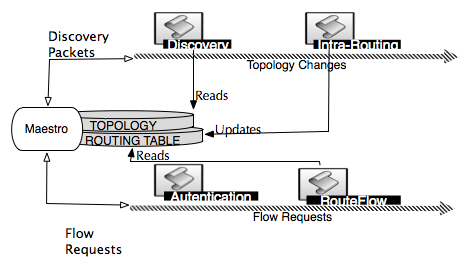
\includegraphics[scale=0.5]{pic/maestro-pipeline.png}
  \caption[Maestro pipeline]{\textbf{Maestro pipeline} Maestro split the pipeline execution
  into several concurrent pipelines based on the events applications
  process and the state they access or modify. In the figure we can
  see two execution paths: \textbf{Topology Changes} processes the
  events triggered by changes in the Infrastructure and \textbf{Flow
    Requests} processes new flow events.}
  \label{fig:maestro-pipeline}
\end{figure}


The fundamental objective of Maestro is to maximize scalability in a
centralized control plane. To do so it attempts to exploit
parallelization in the controller server. Three major design goals
shape Maestro: fair distribution of work across cores; minimal
overhead introduced by cross-core and cache synchronization and;
minimal memory consumption. In addition, it also
exploits throughput optimization through batching. The results
published show that Maestro linearly scales the throughput with the number of cores
available on the controller. 


Currently Maestro is available under the LGPL 2.1 licence. It ships
with usual switching  and routing capabilities \cite{maestro}.

\subsubsection{Beacon}
\label{sec:beacon}
Beacon is an open source controller built in Java, by David Erickson during his academic studies in Stanford University. 
He is, to our knowledge, the only official maintainer of the
application. 

Beacon is also a Thin Controller with  an event-based programming model. Applications register for
specific type of events and process these  in the order
configured by the user. Any application processing an event chooses to forward the
event further in the pipeline or terminate its execution. It is also
multi-threaded, binding switches to particular threads. Applications receive data from all threads.

Applications in Beacon are implemented as \emph{bundles}. A bundle is the
unit of abstraction in the OSGI \cite{osgi} framework - a component and service
platform for the Java programming language with dynamic capabilities -
allowing features such as \emph{hot-swapping} (i.e., deploy, start and
stop modules in run time). 
Beacon provides a central service (the registry) for registration of bundles as
services. Each bundle implements a service, exports it to the registry and
other bundles may consume it. Applications events in Beacon take place
through the service abstraction: bundles may register in other bundles as
listeners to be notified when for specific events take place. 
%TODO - reescrever essa ultima frase. 

Beacon does not provide any NIB service. The network state is
decentralized and encapsulated in the bundle abstraction. There are
no persistance  mechanisms also. 

At the time of writing the applications available are the following: 
 learning switch, hub, device manager , topology, layer 2
shortest path routing, arp  proxy, dhcp proxy. 

%\cite{Controllers: Beacon with David Erickson. Open Network Summit
%  http://www.youtube.com/watch?v=tZ3G_FDuMjg}

\subsubsection{Floodlight}
Floodlight is an open source Apache licensed controller. It was
initially forked from Beacon. It  is developed and maintained by an open community of developers that is mainly composed of Big Switch\footnote{A SDN vendor with a commercial
distributed controller named Big Controller \cite{:vn}.} employers. It is written in Java, but applications can either be
implemented in Java, Jython or through the REST service
available in the NOS (with limited functionality). Floodlight is also a Thin Controller. 

Floodlight follows the common event driven
programming model of most  controllers. Although Floodlight was originally
forked from Beacon, the OSGI support was taken for performance and
deployment reasons. The overall functionality is based on modules
(i.e., applications) that implement services that can be consumed by
other modules. It is similar to Beacon in this regard, however the
module/service functionality is directly provided by Floodlight
instead of delegated to a third-party framework as OSGI. 

Floodlight is also multi-threaded. It accomplishes this through an
asynchronous event based multithreaded library named Netty \cite{netty} that manages Input/Ouput communication with the managed
switches. 

Currently the applications available are: topology manager,  link
discovery, forwarding, device manager, storage, firewall and
static flow pusher.  

\subsection{Controller Choice}
In this section we present an overview of relevant centralized
controllers. Centralized controllers are, by our definition, control
planes that do not show any explicit support in the deployment of a
different controllers processes over onde or more servers. 

%TODO - what defines a centralized controller. 
%TODO - pipeline as a common model
%TODO - event based
%TODO - thin. 
\subsection{NOX}
\label{sec:nox}
NOX \cite{Gude:2008jd}  was published and publicly released under
GPL in 2008. It was both developed in C++ and Python. NOX enables a standard interface for the integration of  Management applications 
in the controller. These applications control
network objectives and also cooperate to define the current
network view (i.e., the NIB). The view is shared between applications. One of the
contributions of the article was the definition of the Network
Operating System abstraction for the controller service. However, NOX
is a Thin Controller. 

\begin{figure}
  \centering 
  \footnotesize
  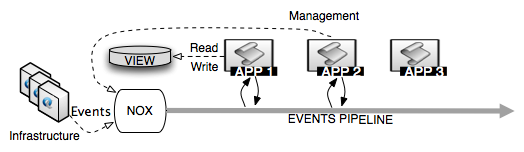
\includegraphics[scale=0.5]{pic/nox-pipeline}
  \caption[NOX pipeline] {\textbf{NOX pipeline} An overview of the NOX
    pipeline used for event processing by the Management applications. NOX
  receives events that have originated either in the Infrastructure of
the Management layer and dispatches them through a pipeline of
applications who have registered for processing these events. 
 As an example: \emph{PACKET\_IN} is a network event while
\emph{USER\_AUTHENTICATED} could be an application event.}
  \label{fig:nox-pipeline}
\end{figure}

NOX is a component framework with primitives for
construction and deconstruction of OpenFlow
based messages. The programming model is event-based. Applications (the components) are registered in a
priority based pipeline with event handlers associated to either
OpenFlow or applications events. This process can be seen in Figure
\ref{fig:nox-pipeline}, which describes the NOX dispatching behavior. Notice
that applications decide if the event should continue to be processed
by the pipeline. NOX  currently ships
with several applications (e.g., forwarding, topology discovery, host
tracking, spanning tree, layer two switch behavior, etc.).

NOX is a centralized controller  but the authors argue that it can easily be distributed for resilience if the shared state (the \emph{view}) is consistently distributed. 
Initially it was a single threaded application not focused on
performance. However, from its publishing date 
several improvements have taken place
\cite{Tootoonchian:2012uia,zen-doc-thesis} that have significantly improved
NOX performance. Under the set of improvements we highlight the
natural evolution to a multi-core aware application
that statically distributes network requests to different threads. 

In the time of writing, NOX is publicly available but has ramified into
two different applications: A C++ based controller available in
Linux and a Python  based controller (POX) available for
several environments \cite{nox}.

\subsection{Maestro}

Maestro is the undergoing work of Zeng Cai covered in
\cite{maestro}. It is presented as a Network Operating System focused
in coordination and isolation of the applications  that control the
infrastructure layer. Cai recognizes that Management components do not
operate independently and in isolation. Instead, they operate
concurrently with inter-dependent state (present in the NIB). With this in mind
it aims to exploit parallell computing benefits in the control plane. 

Maestro splits the regular pipeline execution such that it can
be concurrently executed. As seen in Figure \ref{fig:maestro-pipeline} events may
follow different execution paths since singular control components are
not interested in every single event. Thus, Maestro can manage to
execute several applications concurrently. However, in order to
coordinate the control component access to the NIB Maestro opts to
have a more granular network state model. The author argues that it is
common to control components to be  interested only in  subsets of the
NIB. In order to employ concurrent execution Maestro requires that
applications specify  what subsets of the NIB they require as input
and what subsets they modify as output. 

Maestro employs
coordination of the  execution of the applications with performance in
mind. As an example based on Figure \ref{fig:maestro-pipeline} if the routing table
(subset of the NIB) is updated while the RouteFlow application is running, then
Maestro makes sure that the application will use the old version of
the RoutingTable.

\begin{figure}
  \centering 
  \footnotesize
  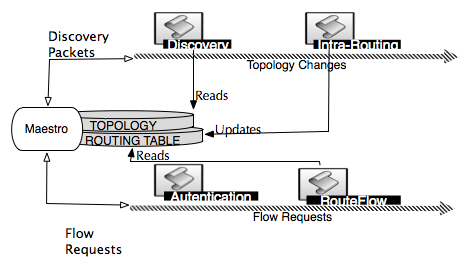
\includegraphics[scale=0.5]{pic/maestro-pipeline.png}
  \caption[Maestro pipeline]{\textbf{Maestro pipeline} Maestro split the pipeline execution
  into several concurrent pipelines based on the events applications
  process and the state they access or modify. In the figure we can
  see two execution paths: \textbf{Topology Changes} processes the
  events triggered by changes in the Infrastructure and \textbf{Flow
    Requests} processes new flow events.}
  \label{fig:maestro-pipeline}
\end{figure}


The fundamental objective of Maestro is to maximize scalability in a
centralized control plane. To do so it attempts to exploit
parallelization in the controller server. Three major design goals
shape Maestro: fair distribution of work across cores; minimal
overhead introduced by cross-core and cache synchronization and;
minimal memory consumption. In addition, it also
exploits throughput optimization through batching. The results
published show that Maestro linearly scales the throughput with the number of cores
available on the controller. 


Currently Maestro is available under the LGPL 2.1 licence. It ships
with usual switching  and routing capabilities \cite{maestro}.

\subsection{Beacon}
\label{sec:beacon}
Beacon is an open source controller built in Java, by David Erickson during his academic studies in Stanford University. 
He is, to our knowledge, the only official maintainer of the
application. 

Beacon is also a Thin Controller with  an event-based programming model. Applications register for
specific type of events and process these  in the order
configured by the user. Any application processing an event chooses to forward the
event further in the pipeline or terminate its execution. It is also
multi-threaded, binding switches to particular threads. Applications receive data from all threads.

Applications in Beacon are implemented as \emph{bundles}. A bundle is the
unit of abstraction in the OSGI \cite{osgi} framework - a component and service
platform for the Java programming language with dynamic capabilities -
allowing features such as \emph{hot-swapping} (i.e., deploy, start and
stop modules in run time). 
Beacon provides a central service (the registry) for registration of bundles as
services. Each bundle implements a service, exports it to the registry and
other bundles may consume it. Applications events in Beacon take place
through the service abstraction: bundles may register in other bundles as
listeners to be notified when for specific events take place. 
%TODO - reescrever essa ultima frase. 

Beacon does not provide any NIB service. The network state is
decentralized and encapsulated in the bundle abstraction. There are
no persistance  mechanisms also. 

At the time of writing the applications available are the following: 
 learning switch, hub, device manager , topology, layer 2
shortest path routing, arp  proxy, dhcp proxy. 

%\cite{Controllers: Beacon with David Erickson. Open Network Summit
%  http://www.youtube.com/watch?v=tZ3G_FDuMjg}

\subsection{Floodlight}
Floodlight is an open source Apache licensed controller. It was
initially forked from Beacon. It  is developed and maintained by an open community of developers that is mainly composed of Big Switch\footnote{A SDN vendor with a commercial
distributed controller named Big Controller \cite{:vn}.} employers. It is written in Java, but applications can either be
implemented in Java, Jython or through the REST service
available in the NOS (with limited functionality). Floodlight is also a Thin Controller. 

Floodlight follows the common event driven
programming model of most  controllers. Although Floodlight was originally
forked from Beacon, the OSGI support was taken for performance and
deployment reasons. The overall functionality is based on modules
(i.e., applications) that implement services that can be consumed by
other modules. It is similar to Beacon in this regard, however the
module/service functionality is directly provided by Floodlight
instead of delegated to a third-party framework as OSGI. 

Floodlight is also multi-threaded. It accomplishes this through an
asynchronous event based multithreaded library named Netty \cite{netty} that manages Input/Ouput communication with the managed
switches. 

Currently the applications available are: topology manager,  link
discovery, forwarding, device manager, storage, firewall and
static flow pusher.  


\section{Distributed Controllers}
\glsresetall
\label{sec:relatedWork:distributed}

In this section we provide an overview of Distributed Controllers
existent in the literature. By our definition an distributed
controllers provides explicit support to the deployment of several
controller processes over one or more servers. 

\subsection{HyperFlow}
Motivated by the lack of scalability in centralized controllers, HyperFlow \cite{Tootoonchian:2010vy} 
was created as a distributed controller. The 
authors aim was to provide scalability without sacrificing
the simplicity of management applications  in  centralized controllers. It
is built as a \emph{C++} application on top of the NOX 
controller \cite{Gude:2008jd} requiring minor modifications to the
controller core and is not publicly available. 

\subsubsection{Architecture.} HyperFlow is composed of two main components: the controller application
and an event propagation system. The overall architecture can be seen
in figure \ref{fig:hyperflow-design}. The controller component is
an application built on top of NOX \cite{Gude:2008jd} which implements an event logger
responsible for subscribing to OpenFlow events and a command proxy
capable of sending OpenFlow commands to  network devices. In essence
HyperFlow interposes acts as an intermediate layer between NOX and
Management applications. The event
propagation system allows  communication between HyperFlow
instances and  is built over a distributed filesystem. Communication
is done through channels implemented as files. There are three types of channels: the
control channel where controllers advertise themselves; the data
channel where general interest events are published by every
controller;  and finally the individual controller channel for OpenFlow
commands relevant to the controller who owns the channel. The
communication system is based on the well known \emph{Publish/Subscribe}
model  whereby one defines publishers as senders of
messages and subscribers as the receivers. Publishers do not send
messages directly  to receivers.  Instead,
messages are published in a medium (in this case the channels) and
interested receivers subscribe to publishers through some form of
subscription logic (e.g., channel, topics, etc.). The Publish/Subscribe
model allows the decoupling of both space and time in the
communication between publishers and subscribers. 
HyperFlow requires that the communication system  provides:
persistent storage of the events published; \emph{FIFO}
(First-In-First-Out)  ordered delivery of
the messages published by the same controller; and resilience against
network partitioning.

\begin{figure}
  \centering 
  \footnotesize
  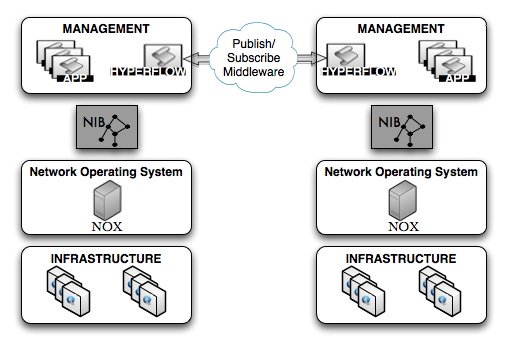
\includegraphics[scale=0.5]{pic/hyperflow-design.png}
  \caption[HyperFlow architecture]{\textbf{HyperFlow architecture} is  similar to
    NOX  with the addition of an Publish/Subscribe middleware
    used between the HyperFlow Management application. The
    Publish/Subscribe system is used for all communication between controllers.}
  \label{fig:hyperflow-design}
\end{figure}


\subsubsection{State Distribution.} State distribution in HyperFlow is accomplished through the
Publish/Subscribe event propagation system. The NIB  is
replicated in all instances and HyperFlow distributes the events
that cause changes to it. This is done through event publishing in the shared
data channel. Every controller subscribes to the
data channel and replays the events received on it, thus changing its
NIB in a similar way.  The view  is maintained by the Management applications
residing in the controller and outside the domain of
HyperFlow (as in NOX). Although not specified in the article HyperFlow attempts to
behave in a similar form to a distributed state machine. However it
lacks total order and does not specify that applications should be
replicated and deterministic. 

HyperFlow does not guarantee strong
consistency as events are not totally ordered  between controllers. 
Notice that even with FIFO based channels some controller $c$ might receive event $e_i$ followed by event
$e_j$ sent from controllers $i$ and $j$, while a controller $c'$
perceives $e_j$ followed by $e_i$. It is possible that such occurrence
leads controllers to divergent states. The article explicitly adverts
that Management applications should not rely in event ordering "except
those targeting the same entity (e.g., the same switch or link)'' as
those guarantee FIFO ordering. 

Additionally, Hyperflow  also addresses incorrectness problems caused by
transient inconsistency across controllers  by defining an
\emph{authoritative}  controller for each flow. This controller is
responsible for orchestrating changes in the network regarding some
flow. As an example, to avoid loop-free forwarding \emph{authoritative}
controllers are solely  responsible for setting the flow paths across the forwarding
plane for some specific flow. For this, applications must relay
requests for some flow to its \emph{authoritative} controller. 

\subsubsection{Scalability.} HyperFlow addresses scalability of the control plane by minimizing the
number of events that an instance replicates to others. Thus it is
focused on the scalability of the CPU and does not address state
scalability since the NIB is fully replicated in every controller. 

To minimize the number of events  processed by
instances, HyperFlow filters the dissemination of events. To this end
it requires that applications tag locally generated events that affect
the NIB. Only these events are worth distributing as others are redundant. 

Local events are generated either by the Management or
Infrastructure layers but Management applications trigger events as a
response to the processing of other events (i.e., there is a causality
relationship between events). Thus, HyperFlow
minimizes distribution of events even further and if, for example,
some event $e$ is triggered due to the processing event $i$, it 
distributes only event $i$. To this end, Management applications
triggering events have to, both flag the event if it affects the NIB state
but also to associate the event that caused it. As one single event
can cause several application events to be triggered this can reduce
the volume of traffic and processing of redundant events.

\subsubsection{Programming Model.} Applications running on HyperFlow act as they control the entire
network. Behind the scenes  HyperFlow redirects requests to the
network equipment  either to the \emph{authoritative} controller or to the
controller managing the equipment which the request addresses. The choice depends on the type of
the request. HyperFlow also routes back  responses to the controller
responsible for  the request. Also, as previously said, every state
changing event is seen by every controller. So in the end the NIB of
the network contains updated information from every  equipment present
in the network.

The programming model itself is identical to NOX  (event driven,
pipeline based) thus
maintains its simplicity. Some overhead complexity is added as
HyperFlow requires the applications to tag  state changing events and
identify parent events as explained above. 

\subsection{Onix}
Onix \cite{Koponen:2010th}  was build upon the NOX legacy and
provides two major contributions: it is the first general controller
published in the literature, and also the first to provide strong consistency.  Onix 
provides an improved Network Operating System interface on 
which the northbound API does not reflect the southbound
API. Management applications are programmed against a network
graph of Typed Entities very similar to the Object Oriented paradigm
and are not aware of the southbound characteristics (e.g., the use of Openflow). The graph is implemented in 
the \emph{Network Information Base}
(NIB) and can be distributed across a  cluster of  Onix
controllers. Applications have the choice to specify consistency and
durability requirements  per network entity  present in the NIB. 
Onix was the result of a joint effort between Google, NEC, Nicira,
ISCI and Berkely, and (at least)  both Google and Ericson have
developed their controllers based on from Onix \cite{The-Valley-of-the-Nerd.:fk}. At the time of
writing Onix is not publicly available. 

\subsubsection{Architecture.} Onix architecture is presented in figure \ref{fig:onix-design}. Only
one application resides on the 
Management layer and may communicate with other applications in other
controllers instances for coordination. The NIB is the
only element in Onix northbound interface. The Management layer
directly modifies the NIB and subscribes to changes on it. The Infrastructure layer
indirectly modifies the NIB (trough the NOS layer). The NOS has to
guarantee that changes in the Infrastructure are reflected in the NIB
and vice versa. For this, it translates network events into changes in
the NIB and changes in the NIB to changes in the Infrastructure configuration. Onix
supports This process is represented in figure
\ref{fig:onix-process}.  OpenFlow but it could transparently move to another
southbound API. 

Each Onix instance  independently manages a subset of the
Infrastructure. However the NIB  exposes all the network for each
instance. As such, each time a local Onix instance alters the NIB these
changes are reflected in all other instances. Thus, the NIB is also
the distribution mechanism of the Onix controller. The  distribution
itself is done by the datastores that back up  the NIB state (seen
in figure \ref{fig:onix-design}).

\begin{figure}
  \centering 
  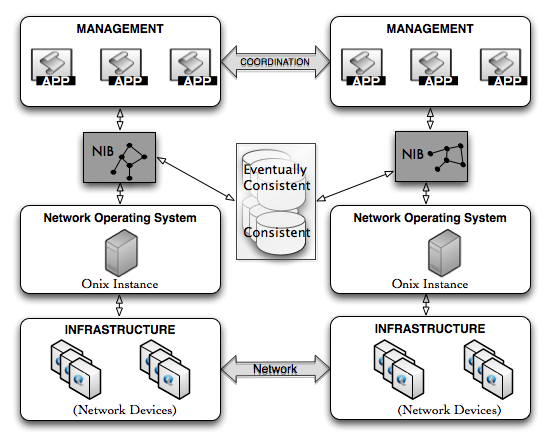
\includegraphics[scale=0.5]{pic/onix-design.png}
  \caption[Onix architecture] {\textbf{Onix achitecture.} In Onix the NIB is the
    solely entity used as the northbound api and Managements program
    directly against it. The NIB is supported by
    two replicated datastores accessible across Onix instances.  The
    Management layer communicates across instances for coordination.}
  \label{fig:onix-design}
\end{figure}

\begin{figure}
  \centering 
  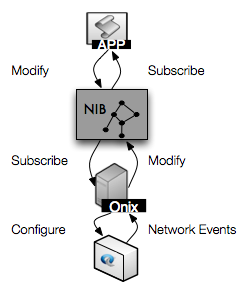
\includegraphics[scale=0.5]{pic/onix-process.png}
  \caption[Onix configuration process]{\textbf{Onix configuration
      process}. The interactions between layers of the Onix
    instance stack. In the figure we can observe the process of
    configuration on the left side, and the process of detecting
    changes in the Infrastructure on the right side.\footnote{The Infrastructure should be only one.}} 
  \label{fig:onix-process}
\end{figure}

\subsubsection{State Distribution.} Onix defines a flexible distribution model for the NIB 
whereby  it offers the application
designer the choice of consistency guarantees. Two
replicated datastores are present, covering  strong 
and  eventually consistency. Strong consistency data is
provided through a transactional persistent database backed up by a replicated
state machine. This datastore is
favored for data with low-frequency changes  as its performance limitations are
significant. The eventually consistent datastore consists in 
an one hop memory based DHT  (as Dynamo 
\cite{DeCandia:2007cn}) favored for  volatile data with high update
rates. 

The NIB reflects the state of both datastores. Both the integration of
datastores and the inconsistency  characteristics of the DHT can lead the
NIB to an inconsistent state where reads performed in some entity may
return more than one result. Thus Onix provides primitives
for the integration of inconsistency resolution logic as well as 
direct integration of a distributed
coordination framework (see  ZooKeeper \cite{Hunt:2010ux}) in the
northbound interface. 

\subsubsection{Scalability.} Onix is intended for large scale Infrastructure where scalability is
fundamental. In each Onix instance the NIB
size reflecting the network state could lead to memory
exhaustion   and the processing of both network events and
subscriptions 
to changes in  the NIB can lead to CPU exhaustion.

In order to introduce scalability and avoid exhaustion, partition and
aggregation based techniques can be configured in the Management
layer. Partition avoids full replication of both data  and workload
such that additional instances do not only replicate overall work but
also relief it. As for aggregation it can, for example, allow network entities to be
aggregated and exposed for other Onix instances as only one.

In practice partition in Onix is present in the division of the
Infrastructure across different Onix instances. 
This way
instances process fewer events. Additionally the Management logic can
configure Onix instances to keep only subsets of the NIB in memory and
up to date. For aggregation, an Onix instance can be configured to
expose a subset of the NIB as an aggregated element. 

\subsubsection{Programming Model.} Applications are built against the NIB graph data structure that is
composed of \emph{Typed Entities} supporting the Object
Oriented paradigm (i.e., encapsulation of data, functions over
entities, hierarchy, etc.). Onix supports extensible representations of
network entities. The
API provides essential functions to search, inspect, create, destroy and
modify entities present in the NIB. It is also possible to register
notifications for creation, removal and updates of data
entities. When network events of other Onix instances update the
datastores those changes must be reflected on the local NIB and the
application must be notified through a callback function. 
All operations are asynchronous, with
eventual delivery and no ordering or latency guarantees given
therefore a \emph{barrier} synchronization primitive is available
allowing the application to wait as
updates are translated and applied in the network devices and/or other
controllers. 

Finally it is worth mentioning that Onix employs coarse-grained
locking mechanisms over the NIB. Applications are given the guarantee
that no other local thread concurrently updates the NIB. 

\subsection{Kandoo}
Kandoo \cite{Yeganeh:2012jm} is an hierarchical controller for
scalable infrastructures. The main
contribution comes from the deployment of isolated controllers near
the switches that shield a parent  controller from processing all
events originating at the network. It is implemented in a mixture of
C, C++ and Python and is not publicly available. 

\subsubsection{Architecture.} In Kandoo --- see Figure  \ref{fig:kandoo-design} --- the controller is split in two levels: in the top level (Network Operating System layer) we
have the root controller responsible for normal operation. In the
bottom (at the Infrastructure layer) we have local controllers that are (ideally)  closer to the
managed switches. This two level design allows  shielding the
controller from frequent events triggered by 
the network devices. Notice that  the entire SDN
stack is replicated in the Infrastructure with the exception of the
NIB since the bottom Management layer should not require direct access to the NIB services. If necessary access to NIB
must be directed to the root controller.

\begin{figure}
  \centering 
  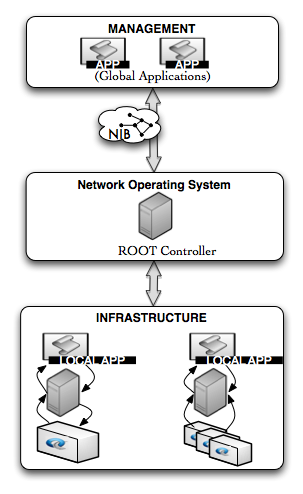
\includegraphics[scale=0.5]{pic/kandoo-design.png}
  \caption[Kandoo design] {\textbf{Kandoo design.} Kandoo decomposes the usual controller
    design into two layers. For this, it brings both controllers and
    applications closer to the Infrastructure. The controllers
    residing in the Infrastructure layer are responsible for
    processing frequent events that do not require access to the
    network state present at the NIB.} 
  \label{fig:kandoo-design}
\end{figure}

This design is motivated by the ideia of bringing control
functionality towards the datapath. As such, \emph{Local Apps} should
require no network wide state and the bottom controllers should stay
close to switches. The deployment of the bottom control plane can
even happen directly at the switches if they support this
functionality (e.g., software switches). 

The remaining design of the controller is not well specified in the
paper. However, other architectures can complement the Kandoo architecture.
The authors stress that even distributing the root
control plane through Onix or HyperFlow is orthogonal to the remaining design.

\subsubsection{Scalability.} In Kandoo scalability is supported by the introduction of the two
level hierarchy. The bottom control plane  shields the root
control from processing of events. As the bottom plane does not
requires access to the NIB it remains simple and
efficient. Additionally, as it is closer to the data plane latency
penalties are lower. However the effectiveness of this
scalability mechanism depends on the Management functionality. For
effective shielding one requires Management applications capable of
operating without access to the network state. The article does not
specifies how practical or significant are this class of
applications beyond exemplifying local policy enforcement  and the
Link Layer Discovery Protocol. 

\subsubsection{Programming Model.} In Kandoo the NOS layer is responsible for the deployment of local
applications in the bottom control plane. The application model only
requires that the applications deployed at the NOS have a flag
that sets its scope (i.e., local or non-local). All the remaining work
is left for the root controller. 

% \subsection{Comparison to Blah, Critic}
% This section is only a scratch for future work orientation. It is
% intended as a comparison to the use of the NIB we are going to build
% and also to criticize the limitations and problems of both HyperFlow
% and Onix. 
% \begin{description}
% \item[TODO] make it clear that HyperFlow replicates controllers. 
% \item[Scalability in Onix] It doesn't exist in the published work (By
%   now it should exist off course). There is quite a bit of blah in the
%   paper about techniques and such but in reality all is left for the
%   application layer to implement relying (again!) on distributed
%   coordination and locking mechanisms; 
% \item[Strong consistency in Onix] Not 100 \% sure about this: it does
%   not exist in practice. If an application mixtures Strong consistency
%   nodes with eventually consistent  links (i.e., (Object A is strong consistent and
%   contains B eventual consistent) it must be prepared to deal
%   with inconsistent resolution upon dealing with the node. The paper
%   suggests this. It is
%   overly complicated in the application logic. 100 \% strong
%   consistency simplifies a lot the application development. 
% \item[Typed entities, Nib Abstraction in Onix] Really cool. higher
%   level of abstraction, another level of indirection. Typed entities
%   combined with the NIB is eternal code loosely coupled to management
%   protocols used in the management of network equipment. Casado
%   defends in a network post
%   [http://networkheresy.com/2011/08/09/what-might-an-sdn-controller-api-look-like-and-should-we-standardize-it/]
%   that it is a general loosely coupled layer, independent of the state
%   distribution mechanism. I disagree, at least in the published
%   work. The state distribution is ``à vista'' in the application layer
%   (define consistency per entity, conflict resolution). It is not
%   fully transparent and consequently not loosely coupled. 

% \item[HyperFlow concept] Kind of reminds a distributed state machine
%   at application level (replay all relevant controller events -i.e.,
%   state changing events) but lacks ordering requirements. 

% \item[HyperFlow] favors availability over consistency. O nosso não
%   fará isso. 
% \item[HyperFlow] sucks. guarantees a bounded window of inconsistency
%   if the network changes trigger less than around 1000 events per
%   seconds. 
% \item[Onix] allows both. The Management deciding. Sacrificing
%   transparency, simplicity. Also, it sucks. 

% \item[Resumo] Hyerflow distribui os eventos o que e estupido porque há
%   muito mais eventos que alteracoes na NIB. Então ele distribui só os
%   eventos que mudam a NIB. O Onix oferece os dois tipos de coerencia
%   mas complica a programacao porque Entities que combinam dois tipos de
%   coerencia podem sempre retornar dois resultados. O Kandoo mete
%   hierarquia ao barulho para minimizar o numero de eventos. 


% \end{description}

\section{Consistent Data Stores}
\glsresetall
\label{sec:relatedWork:consistentDataStore}
%Section data stores do artigo. 
The key idea of our controller architecture is to make the controller instances coordinate their actions through a dependable data store in which all relevant state of the network and of its control applications is maintained in a consistent way.
This data store is implemented with a set of servers (replicas) to avoid any single point of failure, without impairing consistency.
One of the most popular techniques for implementing such replicated data store is state machine replication (SMR)~\cite{Sch90,Lam98}.
In this section we review the state of the art on replicated data stores and describe some reasons why, contrary to common belief, they can be a valid option for supporting a distributed controller architecture.

Practical crash fault-tolerant replicated state machines are usually based on the Paxos agreement algorithm for ensuring that all updates to the data store are applied in the same order in all replicas (thus ensuring consistency)~\cite{Lam98}.
Since the original Paxos describes only an algorithmic framework for maintaining synchronized replicas with minimal assumptions, we instead describe the Viewstamped Replication (VR) protocol, a similar (but more concrete) state machine replication algorithm introduced at the same time~\cite{reitblatt2012abstractions}.
Fig. \ref{fig:paxos} shows the messages exchanged in Paxos/VR for an update operation: the client sends a message to a primary replica (the leader) that disseminates the update to all other replicas. These replicas write the update to their log and send an ACK to the primary.
In the final step the leader executes the request and sends the reply to the client.
If the primary fails, messages will not be ordered and thus a new primary will be elected to ensure the algorithm makes progress.
When read-only operations are invoked, the leader can answer them without contacting the other replicas.
Strong consistency is ensured due to the fact that all requests are serialized by the leader.

\begin{figure}[!ht]
\centering
\includegraphics[width=0.5\textwidth]{pic/related/vr.pdf}
\caption[Paxos/VR update protocol]{Paxos/VR update protocol.} 
\label{fig:paxos} 
\end{figure}

The Paxos/VR algorithm has served as the foundation for many recent replicated (consistent and fault-tolerant) data stores, from main-memory databases with the purpose of implementing coordination and configuration management (e.g., Apache'  Zookeeper~\cite{Hun10}), to experimental block-based data stores or virtual discs~\cite{Rao11,Bol11,Bes13}, and even to wide-area replication systems, such as Google Spanner~\cite{Corbett:2012uz}.
Besides the synchronization protocol, these systems employ many implementation techniques to efficiently use the network and storage media.

Although not as scalable as a weakly consistent data store, these systems grant the advantages of consistency for a large number of applications, namely those with moderate performance and scalability requirements. To give an idea of the performance of these systems, Table \ref{table:smr-results} shows the reported throughput for read and write operations of several state-of-the-art consistent data stores.

\begin{table}
  \center
    \begin{tabular}{ lccc}
    \hline
    \emph{System} & \emph{Block Size} & \emph{kRead/s} & \emph{kWrite/s} \\ \toprule
    Spanner \cite{Corbett:2012uz} & 4kB & 11 & 4 \\ 
    Spinnaker \cite{Rao11} & 4kB & 45+ & 4 \\  
    SCKV-Store \cite{Bes13} & 4kB & N/R & 4.7 \\ 
    Zookeeper \cite{Hun10} & 1kB & 87 & 21 \\ \bottomrule 
    \end{tabular}
  \caption[Performance of state machine replication systems]{Throughput (in thousands data block reads and writes per second) of consistent and fault-tolerant data stores based on state machine replication (N/R = Not Reported).}
  \label{table:smr-results}
\end{table}

Given the differences in the design and the environments where these measurements were taken, we present these values here only as supporting arguments for the possibility of using consistent data stores for storing the relevant state of SDN control applications.
Depending on the specific application this state may include, for instance, a subset of the Network Information Base (NIB).
Interestingly, these values are of the same order of magnitude of the reported values for \emph{non-consistent} updates in Onix (33k small updates per second considering 3 nodes~\cite{koponen2010}), and much higher than the reported values for their consistent data store (50 updates/second for transactions with a single update).
The Onix paper does not describe how its consistent database is implemented but, as shown by these results, its performance is far from what is being reported in the current literature.


\section{Consistent Data Planes}
\glsresetall
\label{sec:relatedWork:consistentPlane}


Recent work on SDN has explored this need for consistency at different
levels. Programming languages such as Frenetic~\cite{Foster2011} offer
consistency when composing network policies (automatically solving
inconsistencies accross network applications' decisions). Other
related line of work~\cite{reitblatt2012abstractions} proposes
abstractions to guarantee data-plane consistency during network
configuration updates. The aim of these systems is to guarantee
consistency \textit{after} the policy decision is
made. Onix~\cite{Koponen:2010:ODC:1924943.1924968} provides a
different type of consistency: one that is important \emph{before} the
policy decisions are made. Onix provides network state consistency ---
both weak and strong --- between different controller instances. The
datastore we propose is similar in that it offers strong consistency
for network (and application) state between controllers\footnote{By
  strong consistency we mean that all accesses to the datastore are
  seen by all controller instances in the same order
  (sequentially).}. Our main objective is to improve the ``performance
limitation''~\cite{Koponen:2010:ODC:1924943.1924968} of Onix's
transactional persistent database. 


Other works on SDN consistency include the Frenetic programming language~\cite{Foster2011}, Reitblatt et al. work on abstractions for network update~\cite{reitblatt2012abstractions}, and Software Transactional Networking~\cite{Canini:2013:HotSDN:STN}. 
These papers address different consistency issues, however. 
In essence, they target consistent flow rule updates on switches, dealing with overlapping policies and using atomic-like flow rule installation in SDN devices.
In other words, they take care of data-plane consistency \emph{after} the policy decisions are made by the network applications. 
Frenetic offers a high level language and a run-time system that, besides other benefits, ensures that policy rules made by concurrent network applications are not overlapped, thus avoiding network inconsistencies.
In~\cite{reitblatt2012abstractions} the authors propose two abstractions --- per-packet and per-flow consistency --- and mechanisms to guarantee that on a network update a packet (or a flow) is processed by exactly one consistent global network configuration. 
STN extends these works by proposing a transactional solution to provide consistent rule installation in a distributed setting. 
Our work targets consistency at a different level.
Our datastore ensures strong control-plane consistency for network and/or applications state, which means policy decisions are always based on a consistent state.